\section{Participant 3}

%%% DK

\subsection{Date \& Time}
\begin{table}[ht]
  \begin{tabular}{|P{3cm}|P{3cm}|}
	\multicolumn{2}{c}{\textbf{2016-08-03}}    	\\ \hline
    Start Time      			& End Time   					\\ \hline
   \textbf{15:38:54} 	& \textbf{15:56:12}    	\\ \hline
   \multicolumn{2}{c}{Duration}    						\\ \hline
   \multicolumn{2}{c}{\textbf{00:17:18}} 			\\ \hline
  \end{tabular}
  \newline\newline
  \caption{P3: Date and Time}\label{dandt3}
\end{table}

\subsection{Questions}
\begin{itemize}
  \item[\Checkmark] Are you a Student?
  \item[\XSolidBrush] Did you work in a team?
  \item[\XSolidBrush] Did you listen to music?
  \item[\Checkmark] Did you feel tired?
  \item[\XSolidBrush] Did you enjoy the tasks?
  \item[\XSolidBrush] Did you give all you attention to the tasks?
  \item[\XSolidBrush] Were you distracted during the tasks?
  \item[\Checkmark] Did you feel stressed
  \item[\XSolidBrush] Do you think the tasks were easy?  
\end{itemize}

\newpage

\subsection{Accelerometer}
\begin{figure}[ht]
	\centering
	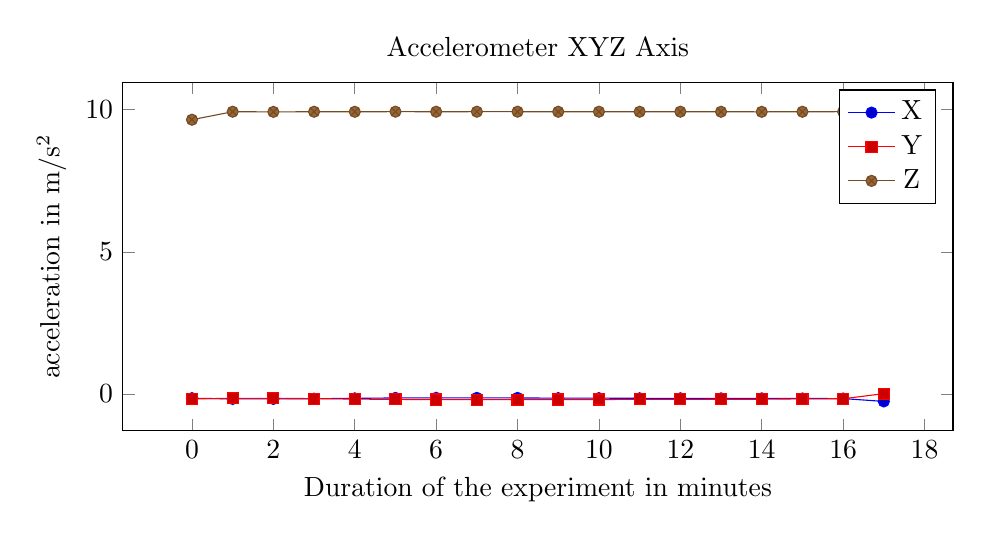
\begin{tikzpicture}
\begin{axis}[
	height=6cm,
	width=\textwidth,
	xlabel=Duration of the experiment in minutes,
	ylabel=acceleration in m/s$^2$,
	title=Accelerometer XYZ Axis,
	unbounded coords=discard],
	
%X
\addplot coordinates {
(0 , -0.144712392571)
(1 , -0.171607927941)
(2 , -0.170622079706)
(3 , -0.162515509394)
(4 , -0.151926182059)
(5 , -0.135589277353)
(6 , -0.132913407353)
(7 , -0.134673849412)
(8 , -0.135671431818)
(9 , -0.144321071176)
(10 , -0.143968983235)
(11 , -0.149250311471)
(12 , -0.150024906176)
(13 , -0.152322015758)
(14 , -0.152559941765)
(15 , -0.156679375)
(16 , -0.158615859706)
(17 , -0.258813207)
};

%Y
\addplot coordinates {
(0 , -0.17022774)
(1 , -0.149285518824)
(2 , -0.151151587353)
(3 , -0.160048757273)
(4 , -0.176325913529)
(5 , -0.187980040294)
(6 , -0.193965545882)
(7 , -0.195585153235)
(8 , -0.195780402121)
(9 , -0.193296577941)
(10 , -0.191571342647)
(11 , -0.185761882941)
(12 , -0.185902718235)
(13 , -0.183047602727)
(14 , -0.180586184118)
(15 , -0.168051834118)
(16 , -0.165798468824)
(17 , 0.01532289)
};

%Z
\addplot coordinates {
(0 , 9.64186077143)
(1 , 9.9233675)
(2 , 9.91780444118)
(3 , 9.92204354545)
(4 , 9.92065644118)
(5 , 9.92477579412)
(6 , 9.92287461765)
(7 , 9.92414205882)
(8 , 9.92422)
(9 , 9.92181826471)
(10 , 9.92354352941)
(11 , 9.92209991176)
(12 , 9.92389579412)
(13 , 9.92153551515)
(14 , 9.91977617647)
(15 , 9.92181838235)
(16 , 9.92442373529)
(17 , 9.9312684)
};

\addlegendentry{X}
\addlegendentry{Y}
\addlegendentry{Z}
\end{axis}
\end{tikzpicture}
	\vspace{5 mm}
\end{figure}

\FloatBarrier

\subsection{Light Level}
\begin{figure}[ht]
	\centering
	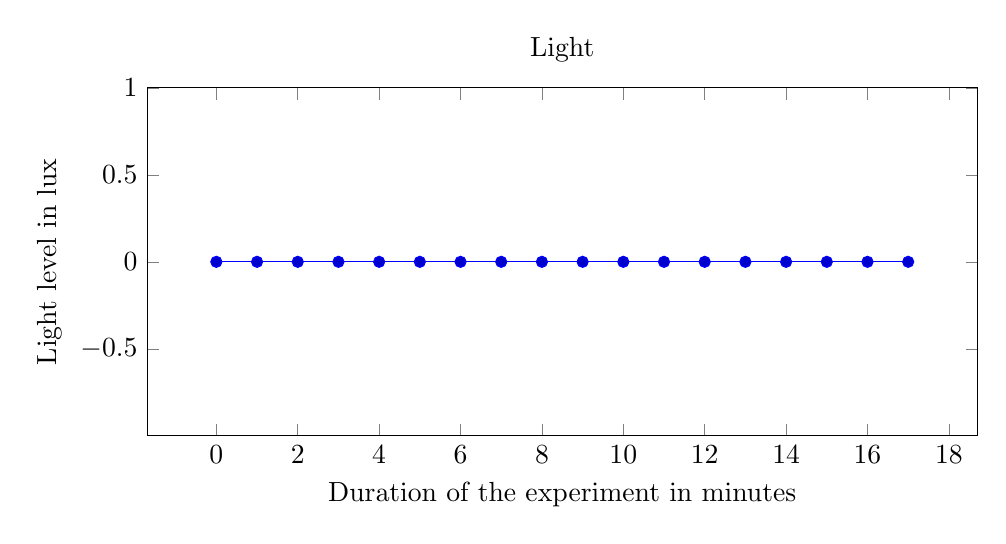
\begin{tikzpicture}
\begin{axis}[
	height=6cm,
	width=\textwidth,
	xlabel=Duration of the experiment in minutes,
	ylabel=Light level in lux,
	title=Light,
	unbounded coords=discard],
	
\addplot coordinates {
(0 , 0.0)
(1 , 0.0)
(2 , 0.0)
(3 , 0.0)
(4 , 0.0)
(5 , 0.0)
(6 , 0.0)
(7 , 0.0)
(8 , 0.0)
(9 , 0.0)
(10 , 0.0)
(11 , 0.0)
(12 , 0.0)
(13 , 0.0)
(14 , 0.0)
(15 , 0.0)
(16 , 0.0)
(17 , 0.0)
};

\end{axis}
\end{tikzpicture}
	\vspace{5 mm}
\end{figure}

\newpage
\FloatBarrier

\subsection{Noise Level}
\begin{figure}[ht]
	\centering
	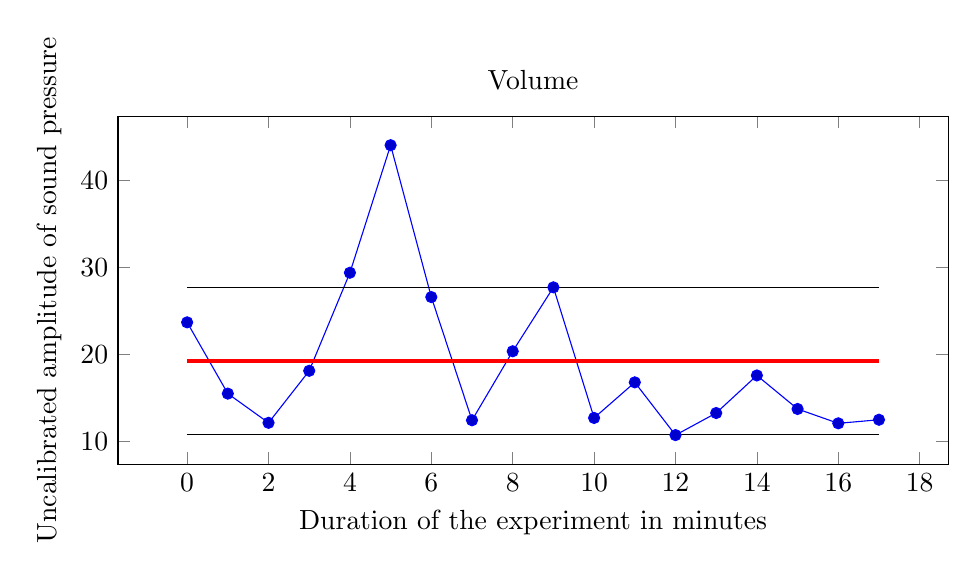
\begin{tikzpicture}
\begin{axis}[
	height=6cm,
	width=\textwidth,
	ylabel=Uncalibrated amplitude of sound pressure,
	xlabel=Duration of the experiment in minutes,
	title=Volume,
	unbounded coords=discard],

\addplot coordinates {
(0 , 23.6857142857)
(1 , 15.5)
(2 , 12.1470588235)
(3 , 18.1212121212)
(4 , 29.3823529412)
(5 , 44.0294117647)
(6 , 26.5882352941)
(7 , 12.4411764706)
(8 , 20.3636363636)
(9 , 27.7058823529)
(10 , 12.7058823529)
(11 , 16.7941176471)
(12 , 10.7352941176)
(13 , 13.2727272727)
(14 , 17.5882352941)
(15 , 13.7352941176)
(16 , 12.0882352941)
(17 , 12.5)
};

\addplot[mark=none, red, very thick] coordinates {(0, 19.2284980302) (17, 19.2284980302)};

\addplot[mark=none, black] coordinates {(0, 10.7687628656) (17, 10.7687628656)};
\addplot[mark=none, black] coordinates {(0, 27.6882331948) (17, 27.6882331948)};

\end{axis}
\end{tikzpicture}
 	\vspace{5 mm}
\end{figure}

\FloatBarrier

\subsection{Location}
No data gathered